
\chapter{深度学习在三维形状分析领域的进展}

随着深度学习的不断发展,不仅在计算机视觉方向取得了巨大成功,而且也被广泛应用于三维形状领域,并且取得了一定的成绩。由于三维形状复杂的拓扑结构和丰富的几何信息,如何将深度学习成功的应用于三维形状领域是一大挑战。为了解决三维形状的识别和检索任务,研究人员们主要沿着如下五个不同的方向进行研究。

\begin{enumerate}
\item 从三维形状中提取描述特征,将其作为深度神经网络的输入,进行学习。
\item 使用目前流行低成本RGB-D相机(Kinect)捕获RGB-D信息,将其作为深度神经网络输入。
\item 直接作用于3D数据的深度神经网络,学习3D形状特征。
\item 利用从不同角度观察三维形状得到的二维图,将三维问题转化为二维问题,之后再利用深度学习方法得到高效的、鲁棒性强的三维形状特征。
\item 深度神经网络作用于超光谱相机拍摄的3D数据。
\end{enumerate}

\section{DL作用于三维模型低层特征}

三维模型低层特征描述符常常被用来进行3D数据的识别检索任务。然而,在三维领域中,由于三维数据的复杂性,通常需要高效率的三维形状描述符。通常的做法是提取的低级别的描述符,之后将他们作为深度神经网络(DNN)的输入,从而使识别和检索任务能有高层次的表现。
\begin{figure}[tb]
\begin{center}
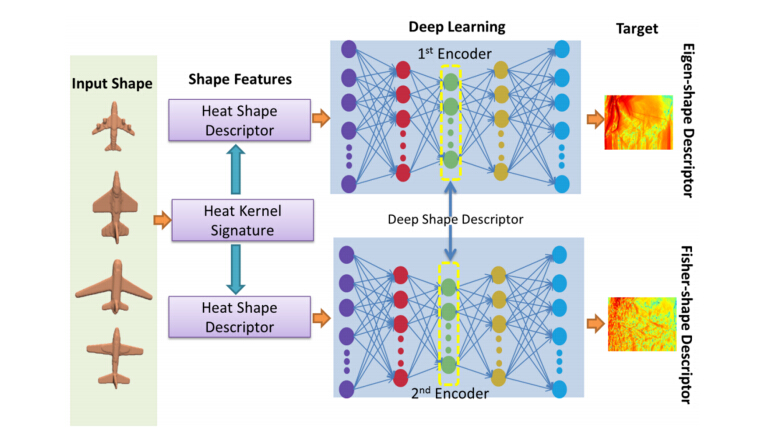
\includegraphics[width=0.9\linewidth]{figures/Fang.jpg} 
\end{center} 
\vspace{-4mm}
\caption{Fang等人提出的三维深度形状特征描述子} 
\label{fig_Fang}
\end{figure}

Liu等人\cite{Liu2014High}采用了深度置信网络(DBN)进行学习3D数据的训练学习,他们采用来自3D数据的底层特征作为DBN的输入数据。具体来说,首先获取每个3D形状的200张深度图像,然后提取每张深度图的SIFT特征描述子。之后,构建BOW字包模型,其中SIFT描述子被编码成BOW模型的``单词''。这些来自三维模型的BOW特征向量,作为DBN的输入数据,对DBN进行逐层的贪婪算法的训练,得到高表达能力的3D特征描述子。该实验同时进行了3D形状的分类和检索实验。实验结果表明该方法获得了比标准BOW模型更为优秀的表现效果,同时证明了在3D数据分析领域深度学习技术具有优秀的效果,并能产生高水平的特征描述子。Bu等人\cite{Bu2014Learning}所作的工作是结合Scale Invariant Heat Kernel Signature (SI-HKS) 和 Average Geodesic Distance (AGD)这两种来自3D数据的局部特征描述子,组成一个低层的3D特征,该特征是由SI-HKS的前6个频率分量和AGD值组成的。接着,一个被称做Geodesics-Aware Bag-of-Features (GA-BoF)的BOW模型的变种被生成。接下来,从GA-BOF中获得的中层特征描述子被用来训练DBN模型,其中DBN的训练采用对比散度的方法。从DBN出来便得到了高层特征描述子。对于3D数据的分类实验中,DBN被认为是一种降维方法,因此他们比较了类似的降维方法,像Principal Component Analysis (PCA) 和 Multi-Dimensional Scaling (MDS)。对于3D模型的检索实验中,DBN模型对比了一些常见的3D数据特征描述子,像Heat Kernel Signature (HKS)。实验结果表明高层特征描述子相较于常见的特征描述子具有更好的可区分性,增强了分类与检索效果。这些被DBN生成的高层特征描述符,又被称做局部深度特征(Local Deep Feature)。在之后的相关工作中,Bu等人利用了基于GPU的深度学习工具包,加快了整个算法的运行速度。

Xie等人\cite{Xie2015Deepshape}将3D形状在不同尺度下的Heat Kernel Signature(HKS)的分布提取出来,用作3D数据的低层特征描述子。这个多尺度的分布特征被用来作为AutoEncoder(AE)深度网络模型的输入,从而获取高层特征描述子。为了提高特征描述子的判别能力,采用了Fisher判别准则。该三维数据的特征表达是由AE的所有激活状态的隐层链接而成。三维形状的匹配和检索实验表明,该高层特征描述子具有鲁棒性对变形不敏感。2015年,Fang等人\cite{Fang20153D}提出了类似的深度学习框架,作者提出的深层三维形状描述符,是利用Heat Shape Descriptor(HeatSD)的方法,该方法是由基于HKS的不同尺度下的形状描述子和多对一的编码器构成。多对一编码器确保了完全相同的输出是由相同类的输入产生。主成分分析(PCA)和线性判别分析(LDA)用于提取三维模型生成特征的形状描述符特征的形状描述符和Fisher的形状描述符(FSD)。预先计算的ESDs和FSDs被作为目标值,分别用来训练两个独立的编码器。该方法同时最大化了类间的边缘和最小化了类内的方差,提高了深度形状特征描述子的判别能力。整个流程图如图\ref{fig_Fang}所示,三维形状特征描述子子在三维形状检索中取得了良好的效果。

\section{DL作用于RGB-D数据}

随着RGB-D传感器逐渐普及,像微软的Kinect传感器,人们可以轻易的获得大量的三维形状的RGB-D数据。这种传感器除了提供常见的RGB三通道的颜色信息外,还提供了额外的深度信息,因此许多研究工作利用这些来自三维模型的RGB-D信息处理诸如3D形状识别、检索和语义分割等信息\cite{Sanchez2016A}。

Socher等人\cite{Socher2012Convolutional}首先提出了基于RGB-D数据对三位形状进行分类的方法。提出了卷积与递归神经网络(RNN)相结合,分别处理颜色信息和深度信息的方法。具体来说,首先,利用两个单层的CNNs分别提取RGB图像和深度图像的低层特征描述子。然后,不同的CNNs的输出被输入到不同的RNN模型中去,其中模型的所有权重都是随即初始化的。从RNN中得到的每一个特征最终被合并成一个特征,同时将其带入到一个联合的softmax分类器中。该方法在对家庭中的三维形状分析中具有精确的性能。Couprie等人\cite{Couprie2013Indoor}采用了多尺度的CNN用来对室内的RGB-D场景进行语义分割。该网络能够处理三个不同尺度的深度图像和RGB图像,然后这些分别得到的上采样结果被合并成一个特征,之后被带入到分类器中从而得到分类标签。最终的分类标签同时融合了分类器的预测结果和RGB-D场景的超像素分割的结果。实验表明,这种方法比在这之前的方法更加有效,运行速度更快。Alexandre\cite{Alexandre20123D}探索了在CNNs之间使用迁移学习用来对3D模型进行识别的可能。该方法应用了四个独立的CNN处理RGB-D图像的四个独立的通道信息。四个CNN依次的进行训练,其中将上一个训练好的CNN权重作为下一个CNN的输入。10个类别的3D物体的实验表明,所提出的训练策略可以提高三维形状分析性能。

在Schwarz等人\cite{Schwarz2015RGB}的基于深度CNN网络的迁移学习也是致力于解决RGB-D物体的识别。其架构采用了一个预训练的CNN进行图像分类,同时将颜色和深度信息分开作为输入对CNN进行训练。同时对输入数据进行必要的预处理从而转换成相应的格式。Schwarz认为深度信息方面,应该从一个规范的视角来渲染物体,同时根据据物体中心不同的距离来对深度进行着色。实验使用网络的最后两个FC层的输出作为描述符,而SVMs最终被用来预测被测试对象的类别、实例和姿态。Eitel等人\cite{Eitel2015Multimodal}也提出了解决RGB-D物体识别的方法。其设计了一个两流CNN结构用来RGB-D物体的识别任务。这两个流(一个用于颜色,另一个用于深度)包含五个卷积和两个FC层。两流原本单独训练,随后,他们在之后的FC层和softmax分类器中被融合。 由于用来完成识别任务的两个CNNs的需要预训练才能完成基于ImageNet数据集的物体识别任务,因此对输入数据进行预处理,尤其是深度信息的处理,是非常必要的。像这种将深度信息编码成彩色图像的方法,被实验证明,效果优于当时其他现存方法。此外,一种新的数据增强方案被采用,该方案生成人工噪声模式,并将它们用作额外的训练样本。大量的实验结果表明,所提出的方法在真实场景、噪声场景中的目标识别任务中具有很好的性能。 Feng等人\cite{Feng20163D}提出了一个集成的CAES(如图\ref{fig_Feng}),利用从类似Kinect的相机获取的一张深度图来解决三维形状的检索问题。每个AE都使用SDG在不同的数据库CAD模型上进行训练。由于该查询不同的数据类型(例如,深度数据)对训练数据的比较(例如CAD模型),所有的AES输出结果转发到一个新的层,称为域适应层(DAL),以确定检索排行。实验结果表明,与其他相关方法相比,该方法获得了更好的性能,比如方向梯度直方图(HOG)描述子,使用L2范数或全局AE。 

\begin{figure*}[htbp]
\begin{center}
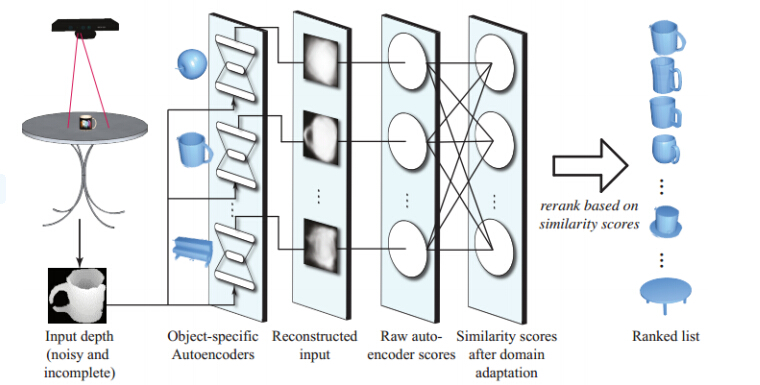
\includegraphics[width=0.9\linewidth]{figures/Feng.jpg} 
\end{center} 
\vspace{-4mm}
\caption{基于深度的压缩自编码器的检索框架} 
\label{fig_Feng}
\end{figure*}

\section{DL作用于3D数据本身}
在过去的几年中,利用捕获场景的完整三维几何图形直接作为DNN的输入的方法已经开始出现。Wu等人\cite{Wu20143D}提出了一种利用整个三维结构实现三维形状表征的新方法。该方法被称为3D ShapeNets,其基本结构为以三维形状作为深度神经网络的输入。这种输入是三维体素网格,这是一种二进制表达,即就是我们认为某个体素网格是否属于该三位形状的一部分。这种体素网格作为之后的DBN的输入,进行训练学习。为了减少与正常分辨率的三维体素量进行全连接时,DBN所需参数数量巨大,于是采用了三维滤波器卷积来降低参数数量。最特别的是,其提出了卷积深度信念网络(CDBN),CDBN一共包含五层,其中三层卷积,一个完全连接层,和一个输出层。该模型首先进行逐层初始化,之后,通过反向传播算法进行微调。标准对比散度被用来训练网络前四层,但更复杂的快速持续对比散度(FPCD)被用于训练网络的顶层。该框架在被用在多种任务,例如三维形状的分类和检索,下一个最好视角预测和基于视图的2.5D的识别任务,在这些任务中都表现优异的效果。此外,作者还发布了ModelNet数据集,这是一个全新的大尺度三维数据集,包括662个不同类型的CAD模型。

Maturana和Scherer\cite{Maturana2015VoxNet}也尝试了使用三维数据的空间表达式进行三维模型的识别方法。如图\ref{fig_Maturana}所示,该VoxNet框架是由体积大小为32×32×32体素网格,该体素网格产生于点云的分割之中,之后将其作为CNN的输入进行训练。该网络架构是由两个带有3D滤波器的卷积,一个池化层和两个全链接(FC)层构成,采用带有动量的随即梯度下降(SGD)的算法进行训练。每一个点云的分割部分,被预测得到一个预测标签。
\begin{figure}[tb]
\begin{center}
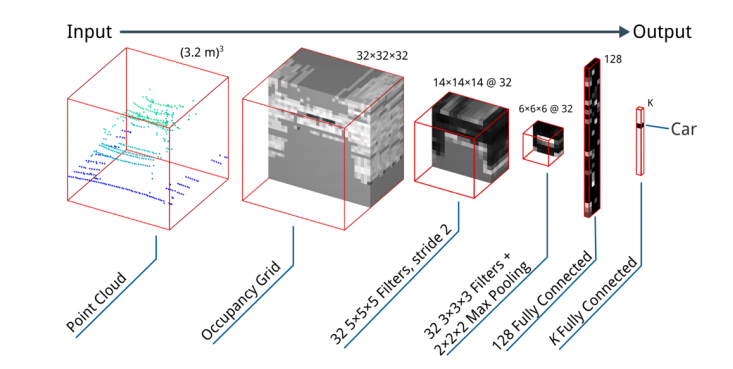
\includegraphics[width=0.9\linewidth]{figures/Maturana.jpg} 
\end{center} 
\vspace{-4mm}
\caption{三维模型的识别的VoxNet4架构} 
\label{fig_Maturana}
\end{figure}
Maturana采用了三个不同领域的三维数据,分别是激光雷达点云数据,RGB-D点云数据和CAD模型,来评价VoxNet模型。实验表明,该框架结构对比同类方法表现更好,同时具有一定的实时性。具体来说,VoxNet的性能表现优于3D ShapeNets\cite{Wu20143D}在三维形状分类的任务中。该实验所采用的数据集是ModelNet10, ModelNet40和NYU v2\cite{Silberman2012Indoor}。另一方面,当使用ModelNet10预训练的模型时,3D ShapeNets在NYU v2数据集上表现更好。 Sedaghat等人\cite{Sedaghat2016Orientation}修改了VoxNet的架构,以便将模型的方向性考虑进去。在最后的模型中,类标签直接从激活的方形中得到。 该方法改进了ModelNet10和其他数据集的分类结果。

Wang等人\cite{Wang2016An}最近提出了一种新的3D描述符学习方法,即卷积自动编码器极限学习机(Convolutional AutoEncoder Extreme Learning Machine, CAE-ELM)。其结合了CNNs, AEs和ELMs的优势。极限学习机(ELM)是Huang等人\cite{Huang2006Extreme}提出的只包含一个隐藏层的前馈网络。ELM的隐含层实际上是固定的和随机的,而输出层是根据感兴趣的任务以监督的方式训练的。Kasun等人\cite{Kasun2013Repre}提出了具有多隐层的标准ELM模型的深入扩展。Wang等人\cite{Wang2016An}提出的架构包括以下几个部分:(i)卷积特征图生成:在这部分网络中,计算三维输入数据(即体素和有符号距离场(SDF)数据)与随机生成的三维内核和卷积特征地图。接下来,为了保持旋转不变性,对特征图应用平均池化。(ii)AE描述符提取:池化之后,每个特征图被作为输入提供给单独的AE。所有的AE最初都是用随机权重初始化的,最后的(输出)权重是通过训练学习的。(iii)ELM分类器:在网络的最后部分,从AE提取的所有描述符被连接成用于预测当前3D形状的标签的矢量。在三维模型分类,三维形状检索和三维形状完成的背景下,CAE-ELM在ModelNet上进行了测试,与Wu等人\cite{Wu20143D}和Xie等人\cite{Xie2015Deepshape}的方法相比,取得了优势。实验中使用的最终体系结构包括两个平行的CAE-ELM层,一个在体素上,另一个在SDF数据上。Han等人\cite{Han2016Mesh}提出了用于从3D网格学习高判别性3D特征的网格卷积限制玻尔兹曼机器(Mesh Convolutional Restricted Boltzmann Machines, MCRBM)。学习得到的特征保留了局部区域之间的结构关系,同时也可以保留局部与全局之间的结构关系。该结构提供了局部区域的新的原始表示,称为局部函数能量分布(Local Function Energy Distribution, LFED),作为对网络的输入。另外,将多个MCRBM组合起来,形成一个更深的模型,命名为网格卷积深度置信网络(Mesh Convolutional Deep Belief Network, MCDBN)。这两种深度模型在进行了全局和局部形状检索和形状对应的情况下,表现了优于诸如BOW,Chen等人\cite{Chen2003On},Kazhdan等人\cite{Kazhdan2003Rotation},Bronstein and Kokkinos等人\cite{Bronstein2010Scale}和Wu等人\cite{Wu20143D}的方法

Qi等人\cite{Qi2016Volumetric}在开创性的工作中,详细阐述了影响体积CNN性能的两个因素,即网络体系结构和体积分辨率,并提出了两种新的CNN体​​系结构,这些体系结构改善了目标分类当前的最新性能,即VoxNet\cite{Maturana2015VoxNet}平均课程准确率达到83%。Lin等人\cite{Lin2013Network}第一个提出的CNN包括的mlpconv层的3D扩展工作,并试图通过包括对对象的部分进行分类的附加学习任务来强调3D物体的细节。这个网络达到了86%的平均分类准确度。第二个CNN最初利用长各向异性核来考虑长距离相互作用,并开发了一个适应性的NIN网络\cite{Lin2013Network}进行分类,平均分类准确率为85.6%。在这两个网络中,还通过应用几个方位角和高程旋转来训练数据增强,同时还使用了多方位池化,从而进一步提高了性能。广泛的实验评估强调了三维分辨率在体积CNN中的重要性。最近,Brock等人\cite{Brock2016Generative}提出了用于形状建模和3D形状分类的基于体素的(全3D)模型,并且与迄今为止提出的任何其他3D或多视图深度学习方法相比,ModelNet10和ModelNet40的大量分类结果得到改善。作者利用了DNN领域的最新进展,并设计了一种网络模型,其依赖于(i)初始式模块的结构\cite{Szegedy2016Inception}(ii)批量标准化\cite{Ioffe2015Batch}(iii)预先激活的剩余联系\cite{He2016Identity}和(iv)随机网络深度\cite{Huang2016Deep}。所提出的模型Voxception-ResNet(VRN)是45层深。作者使用整合VRN模型得到了ModelNet40和ModelNet10的最新分类结果。 应该指出的是,训练如此深的模型需要大量的数据增强。

Song和Xiao\cite{Song2015Deep}提出了一种用于在RGB-D场景中进行3D对象检测和识别的流程,称为Deep Sliding Shapes。有趣的是,Song和Xiao不是使用了深度通道,而是通过使用定向截断有符号距离函数(TSDF)将每个深度图像转换为完整的三维体素网格来利用场景的原始3D信息。然后利用被称为3D区域建议网络(RPN)的完全3D卷积网络,以从两个不同尺度的3D体素网格生成3D对象边界框,以便能够处理不同的对象尺寸。同时还为每个生成的建议对象提议提供了对象分数。此外,每个检测到的3D建议框及其对应的2D色块(即,3D建议框的2D投影)分别被馈送到3D ConvNet和2D ConvNet,以便同时学习物体的类别和3D框回归。对于在三位形状领域的目标评估,该方法优于最先进的选择性搜索方法(Selective Search method)\cite{Uijlings2013Selective},而“深度滑动形状”\cite{Song2015Deep}的目标检测任务与其“非深度”版本相比较,即手工描述符的3D滑动形状\cite{Song2014Sliding}和带有ConvNets描述符的最先进的2D Depth-RCNN\cite{Gupta2014Learning},具有较为优异的性能。


\section{DL作用于3D模型的2D投影/视图}
为了表达3D形状/模型而从不同方向采集的多个2D投影是三维形状分析和理解通常采用的“技巧”。Zhu等人\cite{Zhu2014Deep}通过投影到二维空间来构建3D形状的深度学习的框架,是类似的最早的方法之一。在前面提到的工作中,为了在3D形状检索的应用场景中生成3D形状的全局深度表示,使用了AE。对每个三维模型在位移和尺度方面进行姿态归一化,随后收集他们的一系列二维投影。在用投影预先训练堆叠的RBM之后,使用反向传播对AE进行微调以最小化重建误差。最后,隐藏层用于表示检索过程中3D形状的相应投影/视图。由于每个模型生成不止一个编码(每个投影一个),所以使用Hausdorff距离的变体来计算两个不同3D形状的最终表示之间的距离。实验是在两个流行的数据集进行的,即普林斯顿形状基准(PSB)\cite{Shilane2004The}和工程形状基准(ESB)\cite{Jayanti2006Developing}。结果表明所提出的架构与其他基于全局描述符的方法LFD\cite{Chen2003On}相比表现更好。此外,基于SIFT的BoW这种全局特征与局部特征的线性组合,是性能有所提升。

Leng等人\cite{Leng20153D}利用自编码器实现了三维形状检索的工作。在其工作中,提出了从CNN启发的标准AE的扩展,称为堆叠局部卷积自动编码器(Stacked Local Convolutional AutoEncoder, SLCAE)。局部卷积自动编码器(LCAE)通过使用卷积运算将局部连接的层代替标准AE的FC层而构建。在LCAE的堆叠版本中,许多编码器被放置在彼此的顶部,并且最后一个的输出被用作三维模型的表示。提供给所提出的AE的输入是三维形状的多个视图的多个深度图像,而该架构的每一层都是使用梯度下降法来训练的。堆叠局部卷积自动编码器(SLCAE)与其他优秀的方法在三个三维形状数据集上进行比较,获得了更好的结果。这三个三维形状数据集分别是PSB\cite{Shilane2004The}, 台湾大学数据集(NTU)\cite{Chen2003On}, SHREC'09\cite{Godil2009SHREC}。另外一个叫做3D卷积神经网络(3DCNN)的架构是由Leng等人提出的\cite{Godil2009SHREC}用于同时处理3D对象的多个2D视图。每个形状的视图在被馈送到网络之前被分类成三个合理的序列,以使视图以固定的顺序被列出。3DCNN由四个卷积层,三个子采样层和两个FC层组成。 卷积层最初是以训练AE的相同方式预训练的。之后,整个网络使用反向传播进行了微调。第一个FC层的输出被用作检索的输入数据的表示。对三个数据集(即PSB,NTU,SHREC'09)的评估表明,与其他最先进的方法相比,所提出的方法具有显着的性能。尽管3DCNN表示虽然取得了良好的结果,但是与使用SLCAE\cite{Leng20153D}获得的检索性能相比,在所所使用的3个数据集中其性能性能偏低,这表明后者的表示可能是一个更好的选择来处理三维形状的检索工作。
\begin{figure}[tb]
\begin{center}
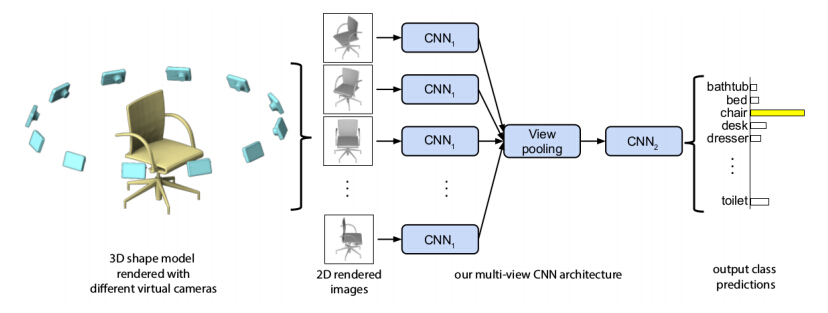
\includegraphics[width=0.98\linewidth]{figures/Su.jpg} 
\end{center} 
\vspace{-4mm}
\caption{MVCNN用于3D对象分类和检索} 
\label{fig_Su}
\end{figure}


Su等人\cite{Su2015Multi}的工作也利用了3D对象的多个视图建立一个紧凑的三维物体分类和检索任务的形状描述符。图\ref{fig_Su}所示的新型多视图CNN(MVCNN)体系结构学习了通过视图池化层将任意数量的对象输入视图组合成一个没有特定顺序的视图。为了获得不同的模型的视图,进行了两步设置。第一个设置包括通过在它们周围放置相同数量的虚拟相机来渲染3D形状得到12个视图,而第二个得到80个视图。三维模型的所有可用视图分别通过网络的第一部分,然后在视图池中的所有视图上执行元素最大池化。最后,汇总的结果通过剩余的网络传递。为了检索,网络倒数第二层(完全连接)被用作形状描述符。在MVCNN架构的实验性评估中,网络使用ImageNet1K数据集进行预训练,然后使用3D数据集ModelNet40进行微调。有关形状分类和检索的报告结果显示MVCNN优于所有其他测试方法。值得注意的是,所提出的形状描述符大大超过了Wu等人\cite{Wu20143D}最先进的3D ShapeNets的性能,特别是使用ModelNet40数据集的检索任务中。Johns等人\cite{Johns2016Pairwise}采用了一种不同的方法来开发3D对象的多个视图针对多视点物体识别在无约束摄像机轨迹下的应用场景。在这项工作中,收集的视图是组织成对,将他们的相对姿势提供给一个CNN。VGG-M网络\cite{Chatfield2014Return}在这种情况下被使用由五个卷积和三个FC层组成。灰度图像,深度图像或二者同时都可以作为网络的输入。结合来自两个图像的卷积层的输出,之后提供给第一FC层。在ModelNet数据集的实验中,这种模型超过了基于体素的3D ShapeNets\cite{Wu20143D}的性能和Su等人\cite{Su2015Multi}的MVCNN方法。

Bai等人\cite{Bai2016GIFT}提出了一种基于3D对象二维视图的实时三维形状搜索引擎。所提出的系统名为GIFT,利用GPU进行基于CNN的特征提取,并利用两个倒排文件,即一个用于加速多视点匹配过程,另一个用于重新排序初始结果。一个查询形状的检索过程能够在一秒钟内完成。作者在ModelNet、 SHREC14LSGTB\cite{Li2015A}、PSB、 McGill\cite{Siddiqi2008Retrieving}、SHREC'07\cite{Giorgi2008SHape}数据集上测试了他们的引擎,均说明了GIFT性能优于较为先进的方法,例如Chen等人\cite{Chen2003On}、Kazhdan等人\cite{Kazhdan2003Rotation}、Wu等人\cite{Wu20143D}和Su等人\cite{Su2015Multi}的方法。Wang等人\cite{Wang2015Sketch}最近提出了一种基于二维草图和二维视图检索三维模型的不同方法。更具体地说,Wang等人提出了一个体系结构,输入是一个对象的{2D视图+草图}对。该模型由两个连体CNN(即两个相同的子卷积网络)组成,一个用于处理要被检索的3D对象的2D草图,另一个用2D视图处理。两个子网分别使用SGD和反向传播进行训练。每一个子网络都包涵三个卷积层(每一个卷积层接一个maxpooling层)、一个FC层加上一个输出层。每个三维模型是被两个随机生成的视图所描述,只要他们的角度差异超过45°。该网络在三个数据集上进行了测试,并取得了最佳性能。

在Leng等人\cite{Leng20143D}所做的工作中,基于视图的深度图像也被用作输入,通过DBN提取高层抽象描述符以用于3D对象分类。DBN使用对比分散的无监督分层训练。。在从训练的DBN获得每个模型的最终表示之后,应用半监督学习方法来对每个对象进行分类。基于准确性和平均分类精度(MCP)的实验评估表明,从提出的DBN中提取的描述符导致相比于两个组合描述符合并得到相当好的结果,组合描述符结合了从不同视图提取的多个2D描述符,即CMVD\cite{Daras2010A}使用图形学习(CMVD-GL)和等权重使用图形融合(EW-GF)。Xie等人\cite{Xie2015Projective}提出了多视点深度极限学习机(MVD-ELM),并对三维形状分类和分割任务进行了测试。每个3D形状由20个2.5D深度图像/投影的集合表示,所述图像/投影使用以每个对象为中心的球体均匀地捕捉。MVD-ELM模型包含卷积层和pooling层。每个卷积层的权重在所有视图之间共享。输出权重根据提取的特征映射进行优化。该模型的完全卷积扩展(FC-MVD-ELM)也被用于三维形状分割任务。这个网络只包含两个卷积层,没有任何pooling层。使用实例的多视点深度图像训练FC-MVD-ELM。然后,将所有预测的标签投影回原始3D网格。最后,使用图形切割优化来平滑分割结果。所提出的模型优于其他相关方法(例如Wu等人\cite{Wu20143D}),并显着减少了训练时间。

受到多视点深度神经网络效果优于采用三维形状的全部三维信息的启发,最近在Qi等人\cite{Qi2016Volumetric}中提出了用于目标分类的体视图与多视图CNN的最近的研究和比较。对于多视图CNN的情况,Qi等人提出了球形渲染,即多分辨率3D滤波以利用多尺度的信息,并结合训练数据增强来实现对已经高性能的MVCNN在ModelNet40数据集上的增强。


\section{DL架构作用于超光谱数据}

先进的遥感技术目前已经被用于多个方面。通常使用机载或星载传感器来捕获超光谱(HS)图像,一般以N个大小为[p1×p2]图像堆叠来表示各个频带的辐射大小,因此也被称为3D超立方体,该方法在Bioucas-Dias等人的文章中可以看到\cite{Bioucas2013Hyperspectral}。传统的HS数据分析方法利用了光谱信息,但也有提出了同时处理光谱和空间数据的方法。最近,应用于HS数据的DL方法开始出现,显示广泛的前景。在Zhang等人\cite{Zhang2016Deep}的研究中,可以找到关于使用遥感数据解决图像预处理,基于像素的分类,目标识别和场景理解的最新DL方法的详细技术教程。在所提到的任务中,基于像素的分类可能是应用最为广泛的。

\begin{figure}[tb]
\begin{center}
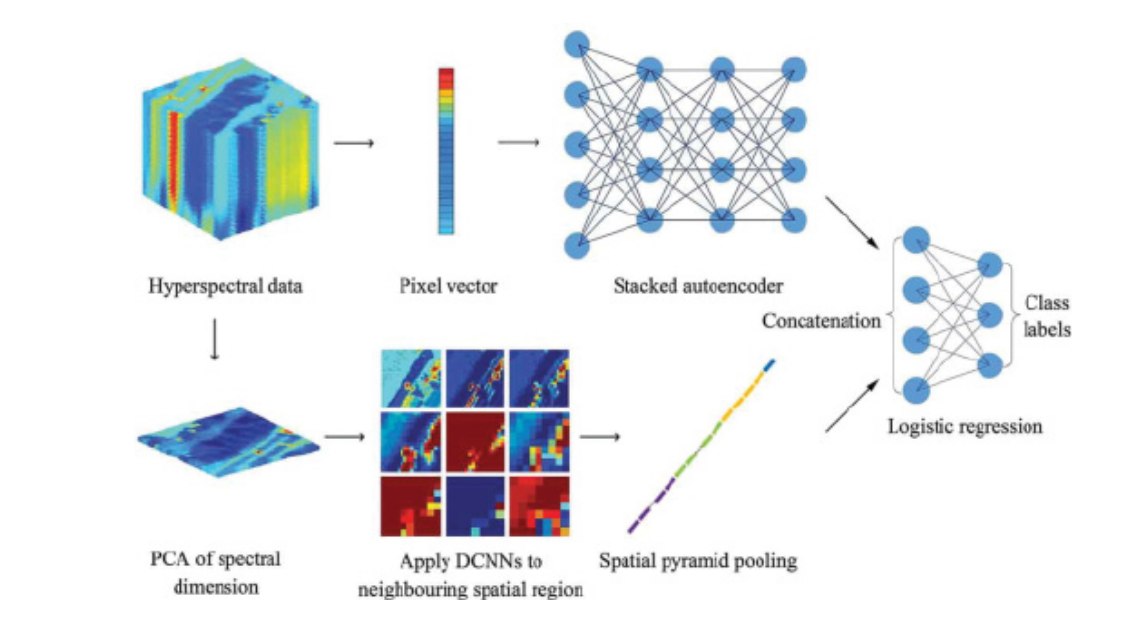
\includegraphics[width=0.9\linewidth]{figures/Yue.png} 
\end{center} 
\vspace{-4mm}
\caption{Yue等人的联合光谱与空间信息的分类框架} 
\label{fig_Yue}
\end{figure}


针对深部高光谱数据分类,Hu等人\cite{Hu2015Deep}采用CNN直接在谱域进行分类。所提出的架构由输入层(接受具有每个像素的频谱的矢量),卷积层,最大池层,FC层和输出层组成。与基于SVM的分类器和其他CNN体系结构相比,作者所提出的方法能够得到更好的结果。在Chen等人\cite{Chen2017Deep}的工作中,其利用堆积AE(SAE)从高光谱数据中提取深度特征来进行分类。作者尝试了两种框架:第一种是利用光谱或空间特征,第二种是基于联合光谱和空间信息特征的分类。具有像素谱的矢量作为AE的输入提取谱特征,而从原始图像中提取特定像素的[n×n]相邻区域并将其作为输入提供给用于空间区域的深度模型得到空间特征。实验结果表明,深度模型比标准SVM分类器表现更好,同时融合光谱特征与空间特征的深度框架比仅使用光谱或空间信息的版本更胜一筹。Chen等人\cite{Chen2015Spectral, Chen2016Deep}提出的类似框架,分别使用DBN和3D CNN的方法也证实了这一观点。Makantasis等人\cite{Makantasis2015Deep}也提出了基于DL的分类方法,其基本思想是利用CNN从光谱和空间数据中提取特征表示。设计的网络包括两个卷积层,而多层感知器用于分类。所提的方法与基于SVM的分类器进行比较,具有明显优势。

Zhou和Wei\cite{Zhou2016Learning}引入了一个称为频谱空间网络(Spectral-Spatial Network,SSN)的分层模型来处理HS图像分类。该网络由几个叠加的光谱空间特征学习单元(SSFLUs)和一个顶层的基于核的极限学习机(KELM)\cite{Huang2012Extreme}组成,并且用于分类。每个SSFLU包括用于提取判别性频谱特征的LDA步骤和用于利用空间信息的自适应加权滤波器(AWF)的应用。与其他最先进的方法相比,实验证明了SSN具有更为良好的准确性和鲁棒性。Zhao和Du\cite{Zhao2016Learning}采用多尺度CNN。该方法首先利用PCA进行降维,然后在三个PC频带上进行特征提取。为每个选定的PC波段构建一个图像金字塔,以多尺度捕捉空间特征。利用Logistic回归(LR)分类器将空间和谱特征相结合来对每个PC带进行分类,而采用投票方案来融合所有谱带的分类结果。作者比较了提出的方法与扩展形态概况(EMPs)\cite{Benediktsson2005Classification}和复合核SVM\cite{Fauvel2012A},并指出其有效性。在Yue等人\cite{Yue2016A}的工作中,空间金字塔池化(SPP)被用于HS图像分类。如图\ref{fig_Yue}所示,DL框架包括将叠加的AE的输出与CNN和softmax分类器组合在一起的特征提取。SPP被应用在深CNN的最后一个卷积层之后,允许产生固定长度的特征而不管输入特征的规模如何。 实验评估结果表明,与RBF-SVM和EMP-SVM相比,该方法性能优越。

\section{总结}
在过去的几年中,DL方法已经被设计并成功应用于一维和二维数据。然而在3D领域使用它们并不那么简单,因为典型的DL架构被设计为将1D或2D数据作为输入。为了克服这个障碍,已经提出了几种方法。在本节中,对于在将数据提供给DL架构之前处理3D数据的方式或者对DL架构进行修改以直接采用3D数据作为输入的方式来识别并分别分析了五个类别。为了处理3D数据,许多研究人员利用了特征工程的进步。低级特征提取已被用于多个计算机视觉任务中,取得了巨大成功,迄今为止已经提出了大量的局部或全局描述符用于3D数据。由于低级描述符通常不足以表征3D对象的高级语义,因此该技术将其与深度模型结合使用,以提取高层描述符。然而,考虑到3D数据的复杂性,这种表示可能缺乏区分能力,因为低层表示可能从3D表示中省略重要的信息。另外,RGB-D传感器的应用能够提供额外的深度模式(除标准RGB通道外),其中包含有关3D对象形状的重要信息。大多数研究者分别处理颜色和深度通道(即图像),而其他人仅使用深度信息来设计他们的系统。这些传感器的巨大优势在于它们对普通用户而言是便宜的,同时还有许多开源软件解决方案可以帮助他们使用。然而,它们的低成本往往与噪声和不完整的捕获数据相结合,可能使得它们不适用于复杂的情况。一些最近的工作已经尝试通过用三维卷积层替换二维卷积层来直接利用三维信息。 3D体积模型提供了丰富而强大的3D形状表示,包括所有重要的细节。尽管在计算硬件方面取得了巨大的进步,但是它们的处理在内存和计算时间方面仍然是要求很高的。结果,低分辨率只被使用到目前为止。其他研究人员从不同的角度来解决这个问题,并利用从不同视点(多视图)捕获的场景的一个或多个2D视图。通过这样做,问题被间接地转换到图像域,因此基于多视图的方法可以利用图像处理的最新进展,并且可以直接使用。然而,它们的使用引起了一些问题:(1)在2D视图中丢失了3D形状的完整的三维几何信息,(2)3D形状的视图的数量以及链接的方式是非常关键的一步,能够影响所提出的方法的效率和有效性。
